\documentclass[11pt,compress,t,notes=noshow, aspectratio=169, xcolor=table]{beamer}

\usepackage{../../style/lmu-lecture}
% Defines macros and environments
% This file is included in slides and exercises

% Rarely used fontstyle for R packages, used only in 
% - forests/slides-forests-benchmark.tex
% - exercises/single-exercises/methods_l_1.Rnw
% - slides/cart/attic/slides_extra_trees.Rnw
\newcommand{\pkg}[1]{{\fontseries{b}\selectfont #1}}

% Spacing helpers, used often (mostly in exercises for \dlz)
\newcommand{\lz}{\vspace{0.5cm}} % vertical space (used often in slides)
\newcommand{\dlz}{\vspace{1cm}}  % double vertical space (used often in exercises, never in slides)
\newcommand{\oneliner}[1] % Oneliner for important statements, used e.g. in iml, algods
{\begin{block}{}\begin{center}\begin{Large}#1\end{Large}\end{center}\end{block}}

% Don't know if this is used or needed, remove?
% textcolor that works in mathmode
% https://tex.stackexchange.com/a/261480
% Used e.g. in forests/slides-forests-bagging.tex
% [...] \textcolor{blue}{\tfrac{1}{M}\sum^M_{m} [...]
% \makeatletter
% \renewcommand*{\@textcolor}[3]{%
%   \protect\leavevmode
%   \begingroup
%     \color#1{#2}#3%
%   \endgroup
% }
% \makeatother


\title{Interpretable Machine Learning}
% \author{LMU}
%\institute{\href{https://compstat-lmu.github.io/lecture_iml/}{compstat-lmu.github.io/lecture\_iml}}
\date{}

\begin{document}

\newcommand{\titlefigure}{figure/feature-effect}
\newcommand{\learninggoals}{
\item Global Feature Effects
\item Local Feature Effects
%\item Understand how to interpret ICE curves and PD plots
}

\lecturechapter{Introduction to Feature Effects}
\lecture{Interpretable Machine Learning}

% \begin{frame}{Feature Effects - Global View}

% %Here,

% %Here, the marginal effect of a feature $x_j$ does not vary across observations and is quantified by its associated coefficient $\hat\theta_j$. %, which explains how a feature affects the model prediction.

% %The $\hat\theta$-coefficients are constant across different observations.
% %It is sufficient to consider a feature's $\hat\theta$ coefficient as marginal effect as it provides an understanding how a feature affects the model prediction. % on average.

% %\lz
% % \textbf{Example}: %Visualizing the marginal effect of a LM (left) and a GAM (right) with a single feature (temperature) to predict the number of bike rentals.
% % Feature effect of LM (left) visualizes relationship of a single feature (here: temperature) on prediction (here: number of bike rentals) while ignoring all other features.
% % GAM (right) replaces linear terms $x_j\hat\theta_j$ of LM by non-linear functions $f_j(x_j)$ estimated via splines.
% %Marginal effects of a LM with features temperature (\texttt{temp}) and \texttt{season} to predict the number of bike rentals (\texttt{cnt}).

% \centering
% %\includegraphics[width=0.75\textwidth, trim=0cm 0.56cm 0cm 0.08cm, clip]{figure_man/lm_main_effects}

% \includegraphics[width=0.375\textwidth, trim=0cm 0.1cm 10.4cm 0cm, clip]{figure/lm_main_effects}\phantom{\includegraphics[width=0.375\textwidth, trim=10cm 0.1cm 0.4cm 0cm, clip]{figure/lm_main_effects}}

% LM without interaction: $\hat\theta_j$ is linear effect of feature $x_j$ (applies globally to all observations):
% %the prediction of any observation $\xi$ is %can be expressed by %explained by its marginal feature effects
% %prediction of an observation $\xi$ can be explained by the individual main effects, e.g.:
% $$\fh(\xv) = \hat\theta_0 + x_1\hat\theta_1$$ % + \dots + x_p\hat\theta_p.$$

% %\phantom{\includegraphics[width=0.375\textwidth, trim=0cm 0.1cm 10.4cm 0cm, clip]{figure/lm_main_effects}}\includegraphics[width=0.375\textwidth, trim=10cm 0.1cm 0.4cm 0cm, clip]{figure/lm_main_effects}

% % \begin{tabular}{c@{}c}
% %  \includegraphics[width=0.4\textwidth,trim=0cm 0.1cm 10.4cm 0cm,clip]{figure/lm_main_effects}\pause% 
% % &\includegraphics[width=0.4\textwidth,trim=10cm 0.1cm 0.4cm 0cm 0,clip]{figure/lm_main_effects}
% % \end{tabular}
% \end{frame}


\begin{frame}{Feature Effects - Global View}
%\includegraphics[width=0.375\textwidth, trim=0cm 0.1cm 10.4cm 0cm, clip]{figure/lm_main_effects}\phantom{\includegraphics[width=0.375\textwidth, trim=10cm 0.1cm 0.4cm 0cm, clip]{figure/lm_main_effects}}

\begin{columns}[T, totalwidth=\textwidth]
\begin{column}{0.49\linewidth}
\includegraphics[width=0.85\textwidth, trim=0cm 0.1cm 10.4cm 0cm, clip]{figure/lm_main_effects}

\bigskip
LM without interaction: $\hat\theta_j$ is linear effect of feature $x_j$ (applies globally to all obs.):
\begin{itemize}
    \item Model equation: $\fh(\xv) = \hat\theta_0 + x_1\hat\theta_1$
    \item Scalar $\hat\theta_1$ describes global effect
\end{itemize}
%$$% + \dots + x_p\hat\theta_p.$$
\end{column}\pause
\begin{column}{0.49\linewidth}
\invisible<1>{\includegraphics[width=0.85\textwidth, trim=10cm 0.1cm 0.4cm 0cm, clip]{figure/lm_main_effects}}

\bigskip
GAM without interaction: $\fh_j(x_j)$ is non-lin. effect of feature $x_j$  (applies globally):
\begin{itemize}
    \item Model equation: $\fh(\xv) = \hat\theta_0 + \fh_1(x_1)$
    \item Curve $\fh_1$ describes global effect
\end{itemize}
%$$% + \dots + \hat{h}_p(x_p).$$
\end{column}
\end{columns}

\end{frame}


\begin{frame}{Feature Effects - Localized View}

\centerline{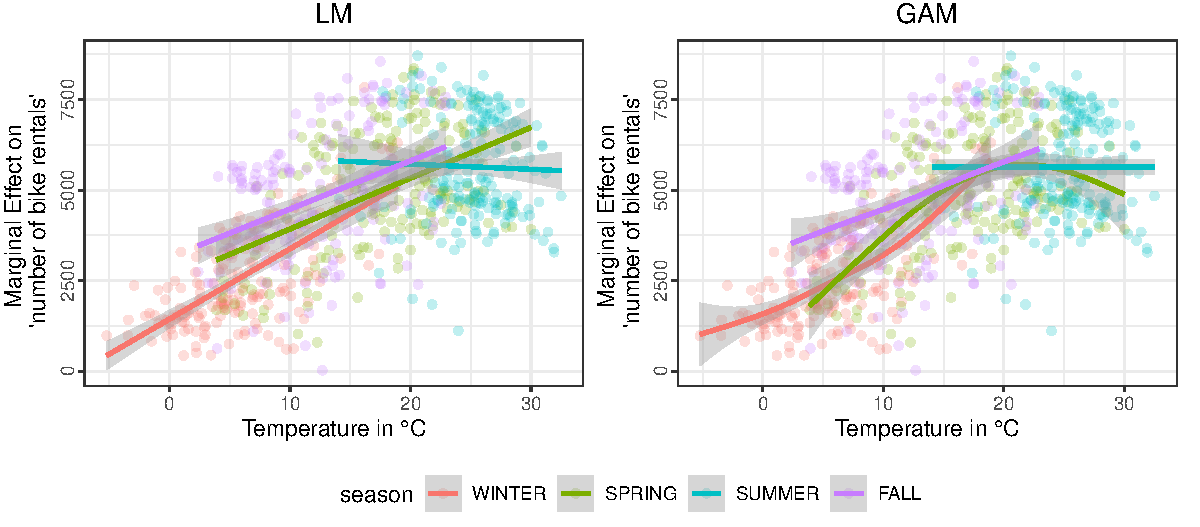
\includegraphics[width=0.8\textwidth, trim=0cm 0.1cm 0cm 0cm, clip]{figure/lm_main_interactions}}

\begin{itemize}
    \item \textbf{Interactions:} Feature effect depends on other features and varies across obs. \\ 
    $\Rightarrow$ E.g., effect of \textbf{temperature} varies across \textbf{season}\\
    $\Rightarrow$ Multiple values / curves needed to describe effect
    \item ML models capture non-linear effects and high-order interactions \\
    $\Rightarrow$ Global view often misleading (single curve may fail to capture complexity)\\
    $\Rightarrow$ Need for local feature effect methods to estimate effects for individual obs.\\
    %Need for local feature effect methods, e.g., analyze effect for individual obs.\\
    $\Rightarrow$ Global view can be reconstructed by aggregating local effects
\end{itemize}

\end{frame}

%
% \begin{frame}{Feature Effects}
%
% %If the model contains interactions, the global effect is not enough as the
% %If the model contains interactions, there is a modifying effect for certain observations that changes the slope of the regression line (in case of LMs) or the shape of the partial effect curve (in case of GAMs).
% %(in case of LMs) or the shape of the partial effect curve (in case of GAMs).
% %If the model contains interactions, the slope of the regression line (in case of LMs) or the shape of the partial effect curve (in case of GAMs) will be different for certain observations.
% If the model contains interactions, the functional shape of the estimated feature effect will usually be different for certain observations.
% \lz
%
% \textbf{Example}: If we include the interaction \texttt{temp*season},
% %the marginal effect of \texttt{temp} will depend on \texttt{season}. That is,
% observations belonging to a certain category of \texttt{season} will have different marginal effects (slopes) for \texttt{temp}.
% %, which results in a different slope for the feature temp at each category of the feature season.
% %so that each category of season yields a different slope for temp.
%
% {\centering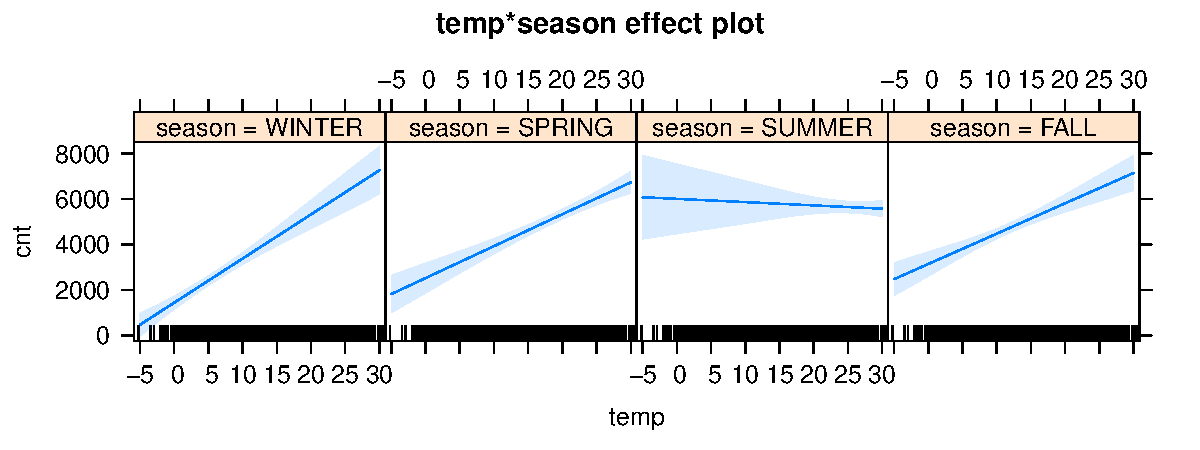
\includegraphics[width=0.9\textwidth, trim=0cm 0.1cm 0cm 0cm, clip]{figure_man/lm_interaction}}
%
% %\textbf{Note}: In case of interactions between two continuous features, we would obtain multiple regression lines with different slopes.
% %The marginal effect can then be visualized in a 2d effect plot or
%
% \end{frame}



\begin{frame}{Feature Effects}

\textbf{Feature effects} visualize or quantify how model predictions change as a single feature varies, while all other features are held fixed.
%marginal contribution of a feature of interest w.r.t. predictions %marginal contribution of a feature to the model \textbf{prediction}. % $\hat{y} = \fh(\xi[])$. effect (e.g., the average relationship) between a
\begin{itemize}
%\tightlist
\item Analogous to regression coefficients (LMs) or Splines (GAMs)
\item Different aggregation levels exist (simplification but information loss)
\item Methods: \visible<1-3>{ICE curves (local curves)}\visible<2-3>{, PD and ALE plots (global curves)}\visible<3>{, AME (global value)}
\end{itemize}

%\centerline{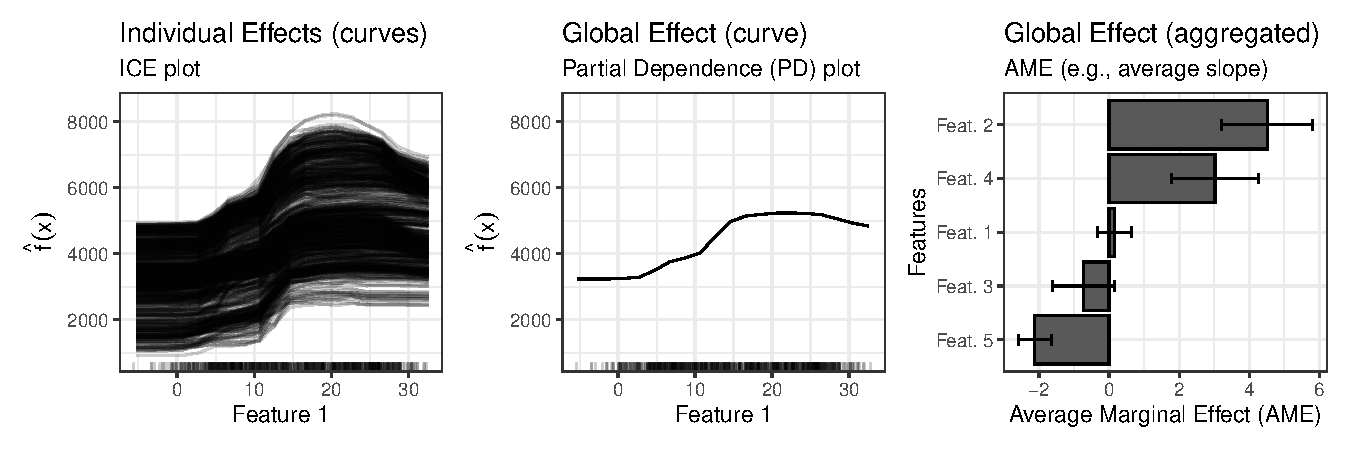
\includegraphics[width=\textwidth]{figure/feature-effect.pdf}}
\centerline{
\visible<1-3>{\adjincludegraphics[width=0.32\textwidth, trim={0 0 {.6667\width} 0}, clip]{figure/feature-effect.pdf}}
\visible<2-3>{\adjincludegraphics[width=0.32\textwidth, trim={{.33\width} 0 {.33\width} 0}, clip]{figure/feature-effect.pdf}}
\visible<3>{\adjincludegraphics[width=0.32\textwidth, trim={{.6667\width} 0 0 0}, clip]{figure/feature-effect.pdf}}
}

\smallskip
%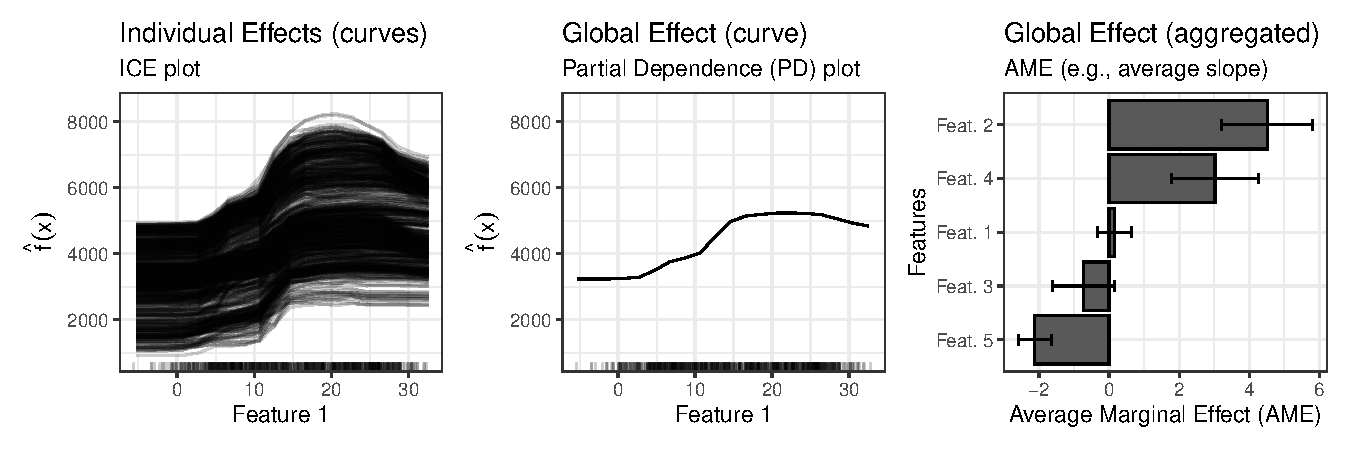
\includegraphics[width=0.33\textwidth, trim=7.4cm 0.1cm 7.4cm 0cm, clip]{figure/feature-effect.pdf}
%\invisible<1>{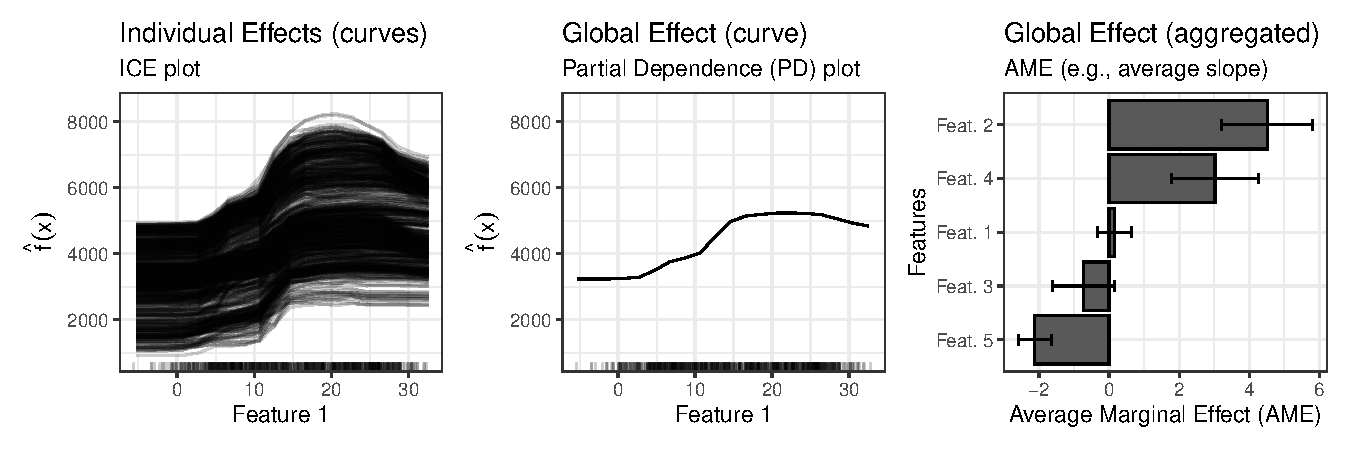
\includegraphics[width=0.33\textwidth, trim=14cm 0.1cm 0.4cm 0cm, clip]{figure/feature-effect.pdf}}

\small  \visible<1-3>{Individual (curves) \hspace{4px}}
\visible<2-3>{$\xrightarrow[\text{curves}]{\text{aggregate}}$ \hspace{4px} Global (single curve)}\visible<3>{\hspace{4px}
$\xrightarrow[\text{slopes}]{\text{aggregate}}$ \hspace{4px} Global (single value)}


\end{frame}


\endlecture
\end{document}
